\section{Results}
\label{sec:results}

Our code and detailed findings, including all evaluated proposals and author verifications, are available at \url{https://anonymous.4open.science/r/AI-Papers-Plagiarism-ECCA}.

\subsection{Expert Evaluation Results}
\label{subsec:expert-evaluation-results}

\begin{table}[t]
    \centering
    \begin{tabular*}{\columnwidth}{@{\extracolsep{\fill}} l cc}
        \toprule
        \textbf{Score} & \textbf{Total Claims} & \textbf{Verified} \\
        & \textbf{(\%)} & \textbf{(\%)} \\
        \midrule
        \textbf{5} & \textbf{18.0\% (9/50)} & \textbf{14.0\% (7/50)} \\
        \textbf{4} & \textbf{18.0\% (9/50)} & \textbf{10.0\% (5/50)} \\
        3 & 32.0\% (16/50) & 8.0\% (4/50) \\
        2 & 28.0\% (14/50) & 4.0\% (2/50) \\
        1 & 4.0\% (2/50) & 0.0\% (0/50) \\
        \bottomrule
    \end{tabular*}
    \caption{Distribution of similarity scores for LLM generated proposals. Considering scores $4$ and $5$ as instances of plagiarism, $24.0\%$ of examined proposals ($36.0\%$ if including unverified claims) are plagiarized.
    We only verify claims for proposals with initial scores of $4$ and above, 
    therefore the total number of verified proposals is less than 50.
    }
    \label{tab:plagiarism-distribution}
\end{table}


Our expert evaluation reveals 
plagiarism in LLM-generated research documents, 
as shown in Table~\ref{tab:plagiarism-distribution}. 
Similarity scores 
across verified claims highlight substantial content misappropriation at various levels of severity. 
Since our evaluation is limited by our participants' time constraints 
and the laborious manual effort required for thorough plagiarism checks, 
our results likely represent a lower bound on actual plagiarism rates. 
Interestingly, 
of the four exemplars presented in \citet{si2024can}, 
one received a similarity score of $5$ 
and another received a score of $4$, 
while among the ten exemplars in \citet{lu2024ai}, 
two received scores of $5$ and one received score $4$---all
of these ratings are cross-verified 
by the source papers' authors.
It is crucial 
to note 
the documents 
that receive similarity
scores of $5$ in our evaluation
passed through SSAG plagiarism detection checks,
indicating serious limitations of such systems (elaborated in §\ref{subsec:automated-plag-exp-results}). 


We also evaluate OpenScholar and Turnitin
on research documents with verified scores of $4$ or above. 
We provided OpenScholar with each document's title, problem statement, motivation section, and methodology section using the prompt shown in Table \ref{tab:openscholar-prompt}. Among the $4$-$5$ papers that OpenScholar suggested as related works for each document, the actual source paper appeared only in one case.
Turnitin did not identify the original paper in any case.
We further analyze these findings through a detailed case study in \S\ref{subsec:case-study}.

\subsection{A Case Study}
\label{subsec:case-study}

\begin{figure*}[t]
    \centering
    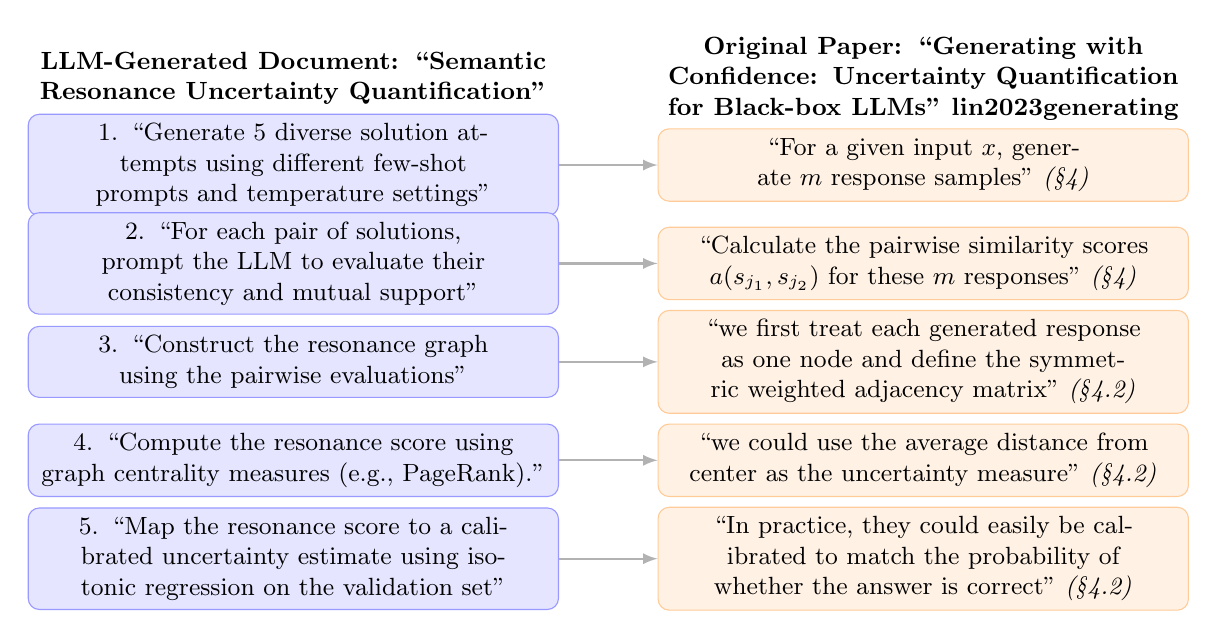
\begin{tikzpicture}[
        box/.style={draw, rounded corners, text width=6.5cm, minimum height=2em, align=center, font=\small},
        leftbox/.style={box, fill=blue!10, draw=blue!40},
        rightbox/.style={box, fill=orange!10, draw=orange!40},
        arrow/.style={->, >=latex, thick, draw=gray!60},
        title/.style={font=\small\bfseries, text width=6.5cm, align=center}
    ]
        \node[title] (t1) at (-4, 3.35) {LLM-Generated Document: ``Semantic \\Resonance Uncertainty Quantification''};
        \node[title] (t2) at (4, 3.35) {Original Paper: ``Generating with \\Confidence: Uncertainty Quantification for Black-box LLMs'' \citep{lin2023generating}};
        
        \node[leftbox] (l1) at (-4, 2.25) {1. ``Generate 5 diverse solution attempts using different few-shot prompts and temperature settings''};
        \node[leftbox] (l2) at (-4, 1) {2. ``For each pair of solutions, prompt the LLM to evaluate their consistency and mutual support''};
        \node[leftbox] (l3) at (-4, -0.25) {3. ``Construct the resonance graph using the pairwise evaluations''};
        \node[leftbox] (l4) at (-4, -1.5) {4. ``Compute the resonance score using graph centrality measures (e.g., PageRank).''};
        \node[leftbox] (l5) at (-4, -2.75) {5. ``Map the resonance score to a calibrated uncertainty estimate using isotonic regression on the validation set''};
        
        \node[rightbox] (r1) at (4, 2.25) {``For a given input $x$, generate $m$ response samples'' \textit{(\S4)}};
        \node[rightbox] (r2) at (4, 1) {``Calculate the pairwise similarity scores $a(s_{j_1}, s_{j_2})$ for these $m$ responses'' \textit{(\S4)}};
        \node[rightbox] (r3) at (4, -0.25) {``we first treat each generated response as one node and define the symmetric weighted adjacency matrix'' \textit{(\S4.2)}};
        \node[rightbox] (r4) at (4, -1.5) {``we could use the average distance from center as the uncertainty measure'' \textit{(\S4.2)}};
        \node[rightbox] (r5) at (4, -2.75) {``In practice, they could easily be calibrated to match the probability of whether the answer is correct''  \textit{(\S4.2)}};
        
        \foreach \i in {1,...,5} {
            \draw[arrow] (l\i) -- (r\i);
        }
    \end{tikzpicture}
    \caption{Visual mapping between an LLM-generated research document (an exemplar in \citep{si2024can}) and a published paper \citep{lin2023generating}, showing a direct correspondence in their proposed methodologies. Each element of the proposed method has a corresponding match in the source paper, suggesting sophisticated rewording rather than novel contribution. This pair receives a similarity score of $5$ in our expert evaluation, which is verified by the authors of the source paper.}
    \label{fig:plagiarism-example}
\end{figure*}

To illustrate the nature of  
plagiarism in LLM-generated research documents, 
we examine a proposal (an exemplar in \citep{si2024can}) 
titled ``Semantic Resonance Uncertainty Quantification'' 
(readers can find this document in their paper). 
This document receives a similarity 
score of $5$ in our evaluation, 
with direct correspondence to an existing published paper, 
``Generating with Confidence: Uncertainty Quantification for Black-box Large Language Models'' \citep{lin2023generating}. 
The authors of the original paper 
confirm our plagiarism assessment 
after reviewing the proposal in question.

As shown in Figure~\ref{fig:plagiarism-example}, 
the proposed methodology exhibits 
a clear one-to-one mapping with the original paper. 
Each component of the LLM-generated 
proposal corresponds to specific sections in the source paper,
albeit with skillfully reworded descriptions. 
The proposal 
proposes the same technical approach 
while using different terminology 
(e.g., ``resonance graph'' instead of ``weighted adjacency matrix'') 
and restructuring the presentation. 
This may be interpreted as adversarial behavior, 
where the LLM has 
learned to disguise existing work as novel research 
through careful rewording. 
Notably, expert reviewers
in \citet{si2024can}'s study 
do not identify this plagiarism, 
likely because 
their evaluation focuses on assessing novelty and feasibility
rather than actively searching for potential sources of plagiarism. 
In contrast, our study's participants, 
operating under different situational logic \citep{popper2013poverty,hoover2016situational} 
that presumes potential plagiarism, 
are able to identify the original paper. 
A similar analysis of plagiarism 
in a showcased paper from \citet{lu2024ai} is provided in
Appendix~\ref{appendix:additional-case}.
This case-study, 
along with results 
of expert evaluation presented in \S\ref{subsec:expert-evaluation-results}, 
showcases the limitations of previous human evaluations of 
LLM generated research ideas---without a skeptical eye for plagiarism, 
experts may be fooled into considering LLM generated research ideas as novel.

\subsection{Performance of Plagiarism Detectors}
\label{subsec:automated-plag-exp-results}

\begin{table}[t]
    \centering
    \small
    \renewcommand{\arraystretch}{1.3}
    \begin{tabular*}{\columnwidth}{@{\extracolsep{\fill}} llr}
        \toprule
        \multicolumn{2}{c}{\textbf{Method}} & \multicolumn{1}{l}{\textbf{Accuracy}} \\
        \midrule
        \multirow{3}{*}{Claude 3.5 Sonnet} & Oracle access & 88.8\% \\
         & Parameteric Knowledge & 1.3\% \\
         & SSAG & 51.3\% \\
        \midrule
        \multirow{3}{*}{GPT-4o} & Oracle access & 89.0\% \\
         & Parameteric Knowledge & 32.7\% \\
         & SSAG & 68.5\% \\
        \midrule
        \multicolumn{2}{l}{OpenScholar} & 0\% \\
        \midrule
        \multicolumn{2}{l}{Turnitin} & 0\% \\
        \bottomrule
    \end{tabular*}
    \caption{Comparing performance of automated plagiarism detectors, including $2$ LLMs in three scenarios (oracle access, parametric knowledge, SSAG), OpenScholar, and Turnitin.}
    \label{tab:model-comparison}
\end{table}

To evaluate automated plagiarism detection methods, we test LLMs in three scenarios (oracle access, parametric knowledge, and SSAG), OpenScholar, and Turnitin. Table~\ref{tab:model-comparison} presents their performance metrics across these settings. Even in our simplified test scenario with deliberately plagiarized proposals, detection accuracy remains remarkably low across all methods.

The oracle access setting, 
where models are given both 
the ground truth paper and plagiarized proposal, 
yields the highest accuracy ($88.8\%$ for Claude 3.5 Sonnet and $89.0\%$ for GPT-4o). 
However, this represents an idealized scenario rarely possible in practice, 
where the source of potential plagiarism is unknown. 
When testing models' parametric knowledge 
without access to external tools, 
GPT-4o achieves notably higher accuracy ($32.7\%$) 
compared to Claude 3.5 Sonnet ($1.3\%$), 
likely because GPT-4o is used to generate these plagiarized proposals in the first place.

The SSAG approach,
a common plagiarism detection method 
in research document generation systems \citep{si2024can,lu2024ai,li2024chain}, 
attains moderate performance ($51.3\%$ for Claude, $68.5\%$ for GPT-4o).
The considerable gap between 
SSAG performance and oracle access 
indicates that retrieving relevant papers, not determining similarity, 
is the bottleneck.

The inadequate performance of SSAG is particularly concerning for research agent systems that rely on it \citep{si2024can,lu2024ai,li2024chain}, especially given our test scenario represents a much easier challenge---our proposals are deliberately plagiarized from single papers, while research agent systems are specifically designed to produce allegedly novel content. (An illustrative example of 
successful plagiarism detection 
using the SSAG
from our synthetic dataset is provided in Appendix~\ref{appendix:successful-detection}.)

Both OpenScholar and Turnitin, 
tested on a smaller subset of proposals ($3$ per topic), 
fail to detect any instances of plagiarism. 
These results, 
combined with significant plagiarism found in our expert evaluation (\S\ref{subsec:expert-evaluation-results}), 
underscore that current automated plagiarism detection methods are inadequate 
for identifying content misappropriation in LLM-generated research documents.

